\documentclass{article}

\usepackage{amsmath,amssymb}
\usepackage{tikz}
\usepackage{pgfplots}
\usepackage{xcolor}
\usepackage[left=2.1cm,right=3.1cm,bottom=3cm,footskip=0.75cm,headsep=0.5cm]{geometry}
\usepackage{enumerate}
\usepackage{enumitem}
\usepackage{marvosym}
\usepackage{tabularx}
\usepackage{multirow}

\usepackage[utf8]{inputenc}

\renewcommand*{\arraystretch}{1.4}

\newcolumntype{L}[1]{>{\raggedright\arraybackslash}p{#1}}
\newcolumntype{R}[1]{>{\raggedleft\arraybackslash}p{#1}}
\newcolumntype{C}[1]{>{\centering\let\newline\\\arraybackslash\hspace{0pt}}m{#1}}

\title{\textbf{Rechtfertigung der Staatstätigkeit, Hausaufgabe 5}}
\author{\textsc{Henry Haustein}}
\date{}

\begin{document}
	\maketitle
	
	\section*{Aufgabe 1}
	\begin{enumerate}[label=(\alph*)]
		\item Es kostet nichts, den Elberadweg zu benutzen, aber es gibt gegenseitige Beeinträchtigung bei Überfüllung
		\begin{align}
			DK &= GZB \notag \\
			4x+20 &= 140 - 4x \notag \\
			x^{priv} &= 15 \notag
		\end{align}
		Optimal wäre es, wenn
		\begin{align}
			GK &= GZB \notag \\
			8x+20 &= 140-4x \notag \\
			x^{opt} &= 10 \notag
		\end{align}
		\item Diagramm
		\begin{center}
			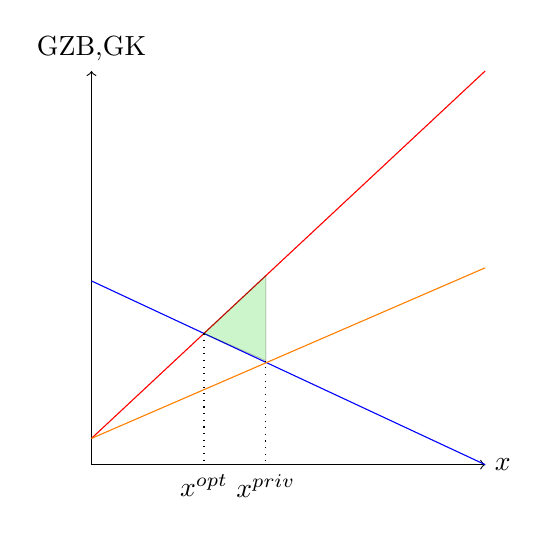
\begin{tikzpicture}
				\draw[->] (0,0) -- (5,0) node[right] {$x$};
				\draw[->] (0,0) -- (0,5) node[above] {GZB,GK};
				
				\draw[blue] (0,7/3) -- (5,0);
				\draw[red] (0,1/3) -- (5,5);
				\draw[orange] (0,1/3) -- (5,2.5);
				
				\draw[fill=green!80!black,opacity=0.2] (10/7,5/3) -- (31/14,1.32) -- (31/14,2.4) -- (10/7,5/3);
				
				\draw[dotted] (31/14,1.32) -- (31/14,0) node[below] {$x^{priv}$};
				\draw[dotted] (10/7,5/3) -- (10/7,0) node[below] {$x^{opt}$};
			\end{tikzpicture} \\
			\textcolor{blue}{GZB}, \textcolor{red}{GK}, \textcolor{orange}{Durchschnittskosten}, \textcolor{green!80!black}{Wohlfahrtsverlust}
		\end{center}
		\item Der Wohlfahrtsverlust ist
		\begin{align}
			WFV &= \frac{1}{2}(x^{priv} - x^{opt})\cdot (GK(x^{priv}) - GZB(x^{priv})) \notag \\
			&= \frac{1}{2}(15-10)\cdot 60 \notag \\
			&= 150 \notag
		\end{align}
		\item Der Preis einer Vignette sollte genau dem Grenzschaden an $x^{opt}$ entsprechen, also
		\begin{align}
			p &= GS(x^{opt}) \notag \\
			&= GK(x^{opt}) - DK(x^{opt}) \notag \\
			&= 100 - 60 \notag \\
			&= 40 \notag
		\end{align}
		Die Stadt wird $x^{opt}$ Vignetten zum Preis von 40 verkaufen. Das erzeugt Einnahmen von 400.
	\end{enumerate}
	
	\section*{Aufgabe 2}
	\begin{enumerate}[label=(\alph*)]
		\item Gesellschaftlich optimal wäre es, wenn die Grenzkosten gleich dem Grenzprodukt sind:
		\begin{align}
			GK &= GP \notag \\
			100 &= 200-10x \notag \\
			x^{opt} &= 10 \notag
		\end{align}
		\item Ohne Zugangsbeschränkung bildet sich die Menge heraus, bei der Durchschnittsprodukt gleich Grenzkosten sind:
		\begin{align}
			GK &= DP \notag \\
			100 &= \frac{200x-5x^2}{x} \notag \\
			100 &= 200 - 5x \notag \\
			x^{priv} &= 20 \notag
		\end{align}
		\item Graph
		\begin{center}
			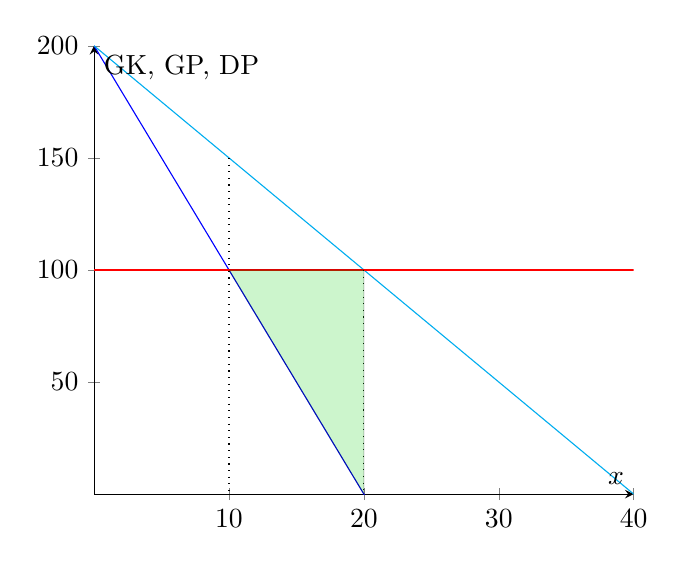
\begin{tikzpicture}
				\begin{axis}[
					xmin=0, xmax=40, xlabel=$x$,
					ymin=0, ymax=200, ylabel={GK, GP, DP},
					samples=400,
					axis x line=middle,
					axis y line=middle,
					domain=0:40,
					]
					\addplot[mark=none,smooth,blue] {200-10*x};
					\addplot[mark=none,smooth,cyan] {200-5*x};
					\addplot[mark=none,smooth,red] {100};
					
					\draw[dotted] (axis cs: 10,150) -- (axis cs: 10,0);
					\draw[dotted] (axis cs: 20,100) -- (axis cs: 20,0);
					
					\draw[fill=green!80!black,opacity=0.2] (axis cs: 10,100) -- (axis cs: 20,0) -- (axis cs: 20,100) -- (axis cs: 10,100);
					
				\end{axis}
			\end{tikzpicture} \\
			\textcolor{blue}{Grenzprodukt}, \textcolor{cyan}{Durchschnittsprodukt}, \textcolor{red}{Grenzkosten}, \textcolor{green!80!black}{Wohlfahrtsverlust}
		\end{center}
		\item Der Wohlfahrtsverlust ergibt sich zu
		\begin{align}
			\text{WFV} &= \frac{1}{2}\big[(GK - GP(x^{priv}))\cdot (x^{priv} - x^{opt})\big] \notag \\
			&= \frac{1}{2} \big[(100-0) \cdot (20-10)\big] \notag \\
			&= 500 \notag
		\end{align}
		\item Der Preis sollte genau der externe Effekt im Optimum sein, dieser ist $DK(x^{opt}) - GP(x^{opt}) = 50$. Es sollten genau $x^{opt}=10$ Lizenzen verkauft werden, die Einnahmen betragen dann $50\cdot 10=500$.
	\end{enumerate}

	\section*{Aufgabe 3}
	\begin{enumerate}[label=(\alph*)]
		\item Zuerst berechnen wir die nötigen Funktionen wie Grenzprodukt und Durchschnittsprodukt:
		\begin{align}
			GP_G &= 20-\frac{G}{2} \notag \\
			DP_S &= 20-\frac{S}{2} \notag \\
			GP_S &= 20-s \notag
		\end{align}
		Es wird sich $GP_G=DP_S$ unter der Nebenbedingung $G+S=30$ einstellen:
		\begin{align}
			GP_G &= DP_S \notag \\
			20-\frac{G}{2} &= 20-\frac{s}{20} \notag \\
			20-\frac{G}{2} &= 20-\frac{30}{2} + \frac{G}{2} \notag \\
			G^{priv} &= 15 \Rightarrow S^{priv}= 15 \notag
		\end{align}
		Damit ergibt sich $GP_G(15)=DP_S(15)=12.5$.
		\begin{center}
			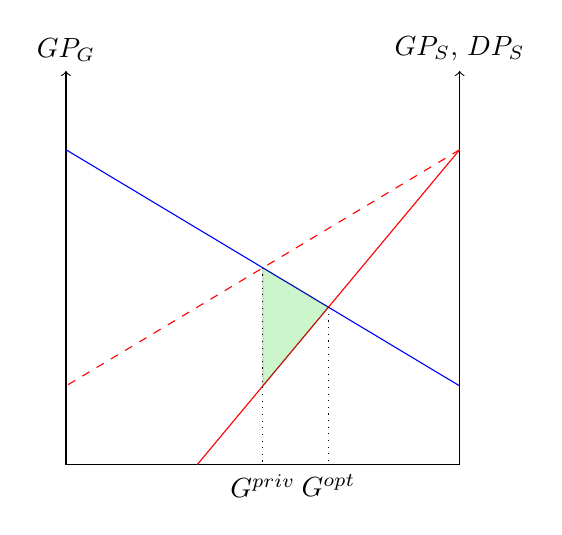
\begin{tikzpicture}
				\draw[->] (0,0) -- (0,5) node[above] {$GP_G$};
				\draw (0,0) -- (5,0);
				\draw[->] (5,0) -- (5,5) node[above] {$GP_S$, $DP_S$};
				
				\draw[blue] (0,4) -- (5,1);
				\draw[red] (5,4) -- (5/3,0);
				\draw[red,dashed] (5,4) -- (0,1);
				
				\draw[fill=green!80!black,opacity=0.2] (2.5,2.5) -- (10/3,2) -- (2.5,1) -- (2.5,2.5);
				
				\draw[dotted] (2.5,2.5) -- (2.5,0) node[below] {$G^{priv}$};
				\draw[dotted] (10/3,2) -- (10/3,0) node[below] {$G^{opt}$};
			\end{tikzpicture} \\
			\textcolor{blue}{$GP_G$}, \textcolor{red}{$GP_S$ bzw. $DP_S$}, \textcolor{green!80!black}{Wohlfahrtsverlust}
		\end{center}
		\item Effizienz wäre es, wenn $GP_G=GP_S$ unter der Nebenbedingung $G+S=30$:
		\begin{align}
			GP_G &= GP_S \notag \\
			20-\frac{G}{2} &= 20-s \notag \\
			20-\frac{G}{2} &= 20-30+G \notag \\
			G^{opt} &= 20 \Rightarrow S^{opt} = 10 \notag
		\end{align}
		Der Wohlfahrtsverlust im Wanderungsgleichgewicht resultiert daher, dass Personen, die in S arbeiten nach G gehen könnten und dort ein höheres Grenzprodukt verdienen könnten, als das Grenzprodukt ihrer Arbeit in S ist.
		\begin{align}
			WFV &= \frac{1}{2}(G^{opt} - G^{priv})(GP_G(G^{opt}) - GP_S(G^{opt})) \notag \\
			&= \frac{1}{2}(20-15)(12.5-5) \notag \\
			&= 18.75 \notag
		\end{align}
		\item Hilfsleistungen nach $S$ treiben $\frac{s}{S}$ nach oben und damit wandern noch mehr Menschen nach $S$. Der Wohlfahrtsverlust wird noch größer. \\
		Bei Einführung von Eigentumsrechten wird nicht mehr $DP_S$, sondern $GP_S$ betrachtet, was zu einer optimalen Lösung führt.
	\end{enumerate}

\end{document}